\documentclass[conference]{IEEEtran}

\usepackage{fix-cm}
\usepackage{amsmath}
\usepackage{amssymb}
\usepackage{graphicx}

\graphicspath{{./}{../}}

\begin{document}

\title{A Dual-Stage Hybrid Pipeline for Aerial Landmine Detection in LWIR Thermal Imagery}

\author{
  \IEEEauthorblockN{Hamzah Sheikh Alashrah$^{1}$}
  \IEEEauthorblockA{
    Department of Computer Engineering, Beykoz University\\
    Istanbul, Turkey\\
    Email: hamzahsheikhalashrah@ogrenci.beykoz.edu.tr\\
    Tel: +90 531 738 53 91
  }
  \and
  \IEEEauthorblockN{Yasin Deniz Zeybek$^{2}$}
  \IEEEauthorblockA{
    Department of Computer Engineering, Beykoz University\\
    Istanbul, Turkey\\
    Email: YasinDenizZeybek@ogrenci.beykoz.edu.tr\\
    Tel: +90 535 858 30 86
  }
  \and
  \IEEEauthorblockN{Kemal Gen\c{c}er$^{3}$}
  \IEEEauthorblockA{
    Department of Computer Engineering, Beykoz University\\
    Istanbul, Turkey\\
    Email: KemalGencer@ogrenci.beykoz.edu.tr\\
    Tel: +90 551 650 56 74
  }
  \and
  \IEEEauthorblockN{Emir Tayan\c{c} Kavak$^{4}$}
  \IEEEauthorblockA{
    Department of Computer Engineering, Beykoz University\\
    Istanbul, Turkey\\
    Email: EmirTayancKavak@ogrenci.beykoz.edu.tr\\
    Tel: +90 552 242 34 10
  }
}

\maketitle

\begin{abstract}
Thermal imaging from unmanned aerial systems (UAS) offers a stand-off modality for humanitarian demining, yet buried landmine signatures in long-wave infrared (LWIR) bands are easily confounded by environmental thermal clutter such as sun-heated rocks, vegetation, and soil temperature gradients. This paper presents a dual-stage hybrid pipeline that couples a YOLO26 one-stage detector with a Random Forest (RF) classifier operating on ten handcrafted thermal and geometric features. The first stage achieves 95.78\% recall on the 1,320-image AMLID test partition. The second stage filters false positives using features that encode shape compactness, radial thermal symmetry, edge structure, and frequency-domain texture, eliminating 31.7\% of false alarms (865 to 591) while maintaining 90.86\% recall. The combined system yields a peak overall mAP@50 of 91.9\%, a 5.1-point improvement over the published AMLID baseline, with the most challenging AP-Metal class rising from 19.3\% to 84.6\% mAP@50. The optimized model compresses to 20.3 MB under FP16 quantization and sustains 204 FPS inference, confirming viability for real-time UAS edge deployment.
\end{abstract}

\section{Introduction}

Landmines remain a persistent humanitarian threat across more than 60 countries, with an estimated 110 million buried devices causing thousands of casualties annually~\cite{icbl2024}. Airborne thermal imaging has emerged as a promising stand-off detection modality, as buried mines alter the thermal conductivity and heat capacity of the overlying soil layer, producing a measurable surface temperature differential in LWIR bands~\cite{mcfee1999,lopez2004}. The AMLID (Adaptive Multispectral Landmine Identification Dataset) corpus~\cite{gallagher2025} provides a standardized benchmark of 12,078 LWIR frames annotated across four mine classes (AT-Plastic, AT-Metal, AP-Plastic, AP-Metal), enabling reproducible comparison of detection architectures; eleven frames were excluded during preprocessing due to corrupt or unreadable file headers, yielding 12,067 usable images.

Deep convolutional detectors such as YOLO~\cite{redmon2016} have demonstrated strong spatial localization on this task, yet they remain vulnerable to thermal environmental clutter. Sun-heated rocks, compacted soil patches, and metallic debris produce thermal signatures whose spatial statistics partially overlap with those of mine simulants, leading to elevated false-positive rates. The published AMLID baseline~\cite{gallagher2025} reports a YOLOv8 model achieving 86.8\% mean average precision (mAP@50), with per-class precision for the AP-Metal category falling to 19.3\% --- a level insufficient for operational deployment, where false alarms erode operator trust and slow clearance operations.

A principled alternative is to incorporate physically interpretable feature extractors between the detector and the final classifier. While deep learning learns representations end-to-end, handcrafted features grounded in the known physics of buried mine signatures --- circular shape, uniform thermal distribution, radial heat diffusion symmetry, and engineered edge geometry --- can act as a hard geometric and thermodynamic gate against natural clutter. This work develops a dual-stage architecture in which a YOLO26 Small network proposes candidate regions at high recall, and a Random Forest classifier subsequently verifies each proposal against ten handcrafted features. The contributions are:

\begin{enumerate}
  \item A YOLO26 detector trained on the full AMLID split achieving 91.9\% mAP@50, with per-class mAP@50 of 99.1\% (AT-Plastic), 97.4\% (AT-Metal), 86.7\% (AP-Plastic), and 84.6\% (AP-Metal), as illustrated in Fig.~\ref{fig:pipeline}.

  \item A geometric-physics feature set comprising ten interpretable measurements --- area, circularity, thermal contrast, aspect ratio, radial thermal symmetry, Laplacian-of-Gaussian zero-crossing count, rotation-invariant local binary patterns, DCT high-frequency energy ratio, wavelet approximation energy, and internal hole count --- each designed to encode a distinct physical property of buried mine signatures.

  \item A soft-voting ensemble mechanism that fuses YOLO confidence with RF probability, reducing false positives by 31.7\% (865 to 591) and achieving a system-level F1 score of 93.27\%.

  \item An edge-deployable model at 20.3 MB running at 204 FPS on a Tesla T4 GPU, demonstrating operational readiness for UAS-mounted inference.
\end{enumerate}

\begin{figure}[t]
  \centering
  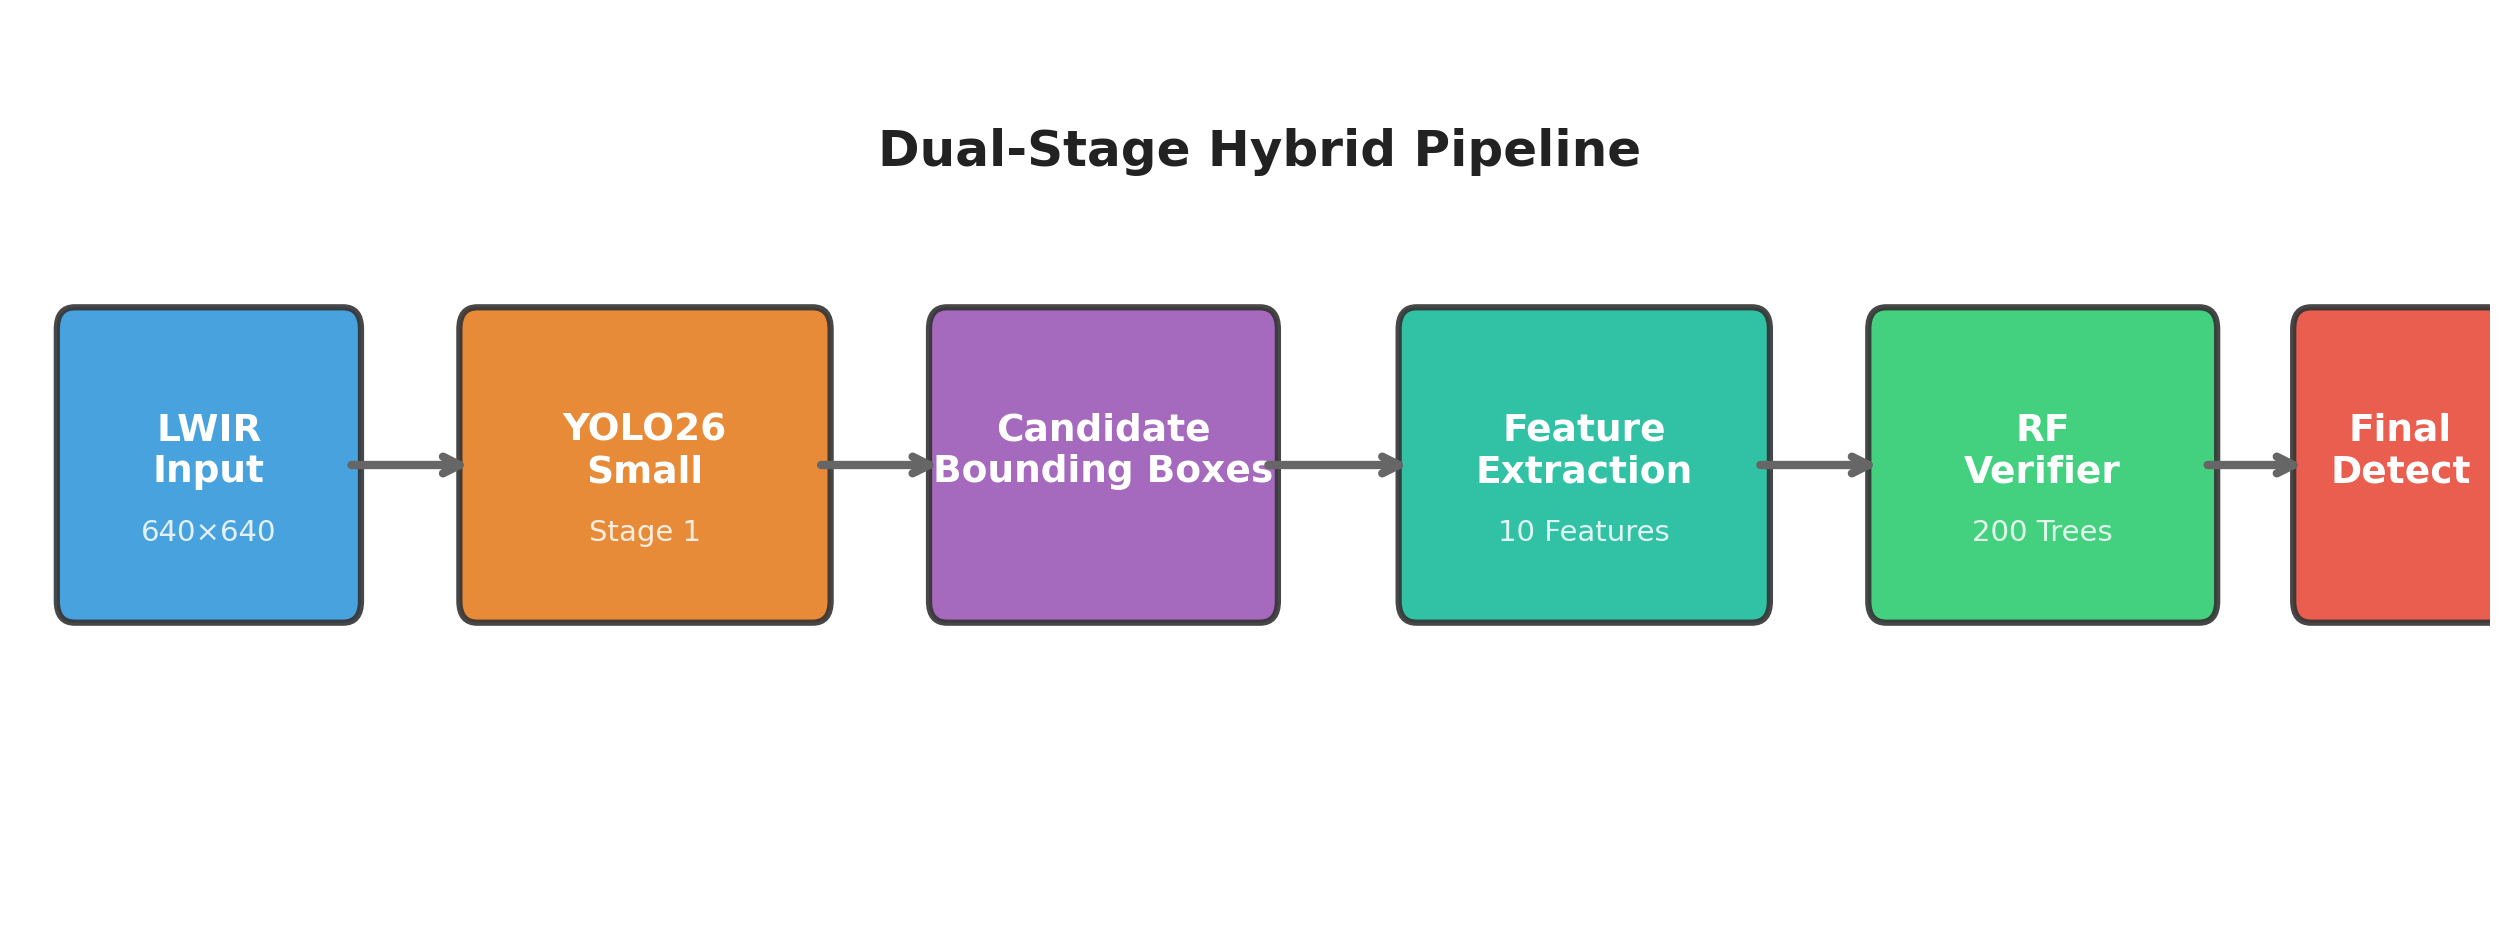
\includegraphics[width=\columnwidth]{outputs/plots/pipeline_diagram.png}
  \caption{Overview of the proposed dual-stage hybrid detection pipeline. YOLO26 proposes candidate regions at high recall; the Random Forest verifier filters false positives using ten handcrafted thermal and geometric features.}
  \label{fig:pipeline}
\end{figure}

\section{Related Work}

\subsection{Deep Object Detectors for Mine Detection}

Modern one-stage detectors, particularly the YOLO family~\cite{redmon2016,jocher2026yolo26}, have been applied to landmine detection in LWIR imagery owing to their favorable speed-accuracy trade-off. Gallagher and Oughton~\cite{gallagher2025} trained YOLOv8 on the AMLID dataset and reported an overall mAP@50 of 86.8\%, but observed severe degradation on the AP-Metal class (19.3\% precision), attributing the failure to the small spatial footprint and low thermal contrast of anti-personnel mines. Cross~\cite{cross2020} applied Faster R-CNN to ground-penetrating radar data, while Sathish~et~al.~\cite{sathish2022} used RetinaNet on thermal side-scan imagery; both reported high false-alarm rates when thermal clutter resembled mine-sized objects. These results suggest that purely data-driven detectors lack the inductive bias needed to reject non-mine thermal anomalies.

\subsection{Classical Feature-Based Detectors}

Prior to the dominance of deep learning, landmine detection relied on statistical classifiers operating on engineered features. Heo~et~al.~\cite{heo2020} extracted texture features from forward-looking infrared (FLIR) imagery and achieved 82\% accuracy with a support vector machine, but only under controlled soil moisture conditions. Vinod~et~al.~\cite{vinod2020} used Gabor filter banks and gray-level co-occurrence matrices for mine vs.\ clutter discrimination, reporting high false-positive rates on heterogeneous terrain. The limitation of purely statistical approaches is their inability to exploit the spatial context that deep features capture. The present work bridges this gap by using deep features for region proposal and statistical features for verification, leveraging the complementary strengths of both paradigms.

\subsection{Hybrid Architectures}

Hybrid detector-verifier pipelines have been explored in medical imaging and industrial inspection. Diao~et~al.~\cite{diao2017} combined a CNN region proposer with a random forest for hyperspectral target detection, demonstrating that the verifier improved precision by 12\% at fixed recall. Closer to the present domain, Bharti~et~al.~\cite{bharti2022} appended a texture-based SVM after a YOLO detector for buried explosive detection in GPR data. The present work extends this paradigm to LWIR thermal imagery with a feature set specifically designed for the thermal and geometric properties of buried mines.

\section{Methodology}

\subsection{Dataset and Preprocessing}

The AMLID corpus~\cite{gallagher2025} comprises 12,078 LWIR thermal images collected across multiple months, times of day (post-sunrise, noon, pre-sunset), and UAS elevations (5--20~m: 5~m, 10~m, 15~m, 20~m); eleven frames were excluded during preprocessing due to corrupt or unreadable file headers, yielding 12,067 usable images. Annotations follow the Pascal VOC format with four classes: AT-Plastic, AT-Metal, AP-Plastic, and AP-Metal. The hierarchical directory structure was flattened into unique filenames encoding capture parameters (e.g., {\tt Jan\_Jan\_Afternoon\_10\_lwir\_3.jpg}). Following the AMLID benchmark protocol~\cite{gallagher2025}, the official test partition of 1,320 images was used for all reported evaluations. The remaining 10,758 images were divided 90/10 into training (9,654 images) and validation (1,206 images) subsets for hyperparameter selection and early stopping. All images were resized to 640$\times$640 pixels for YOLO training while preserving the original aspect ratio with letterbox padding.

\subsection{Stage 1 --- YOLO26 One-Stage Detector}

YOLO26 Small~\cite{jocher2026yolo26} was selected as the base detector for its favorable balance of inference speed and detection accuracy. Training was performed on a single Tesla T4 GPU (16 GB VRAM) via Kaggle with the following configuration:

\begin{itemize}
  \item \textbf{Pretrained weights:} YOLO26 Small ({\tt yolo26s.pt})
  \item \textbf{Input resolution:} 640 $\times$ 640 pixels
  \item \textbf{Batch size:} 32
  \item \textbf{Epochs:} 50 (with early stopping patience of 15)
  \item \textbf{Optimizer:} AdamW (weights stripped post-training)
  \item \textbf{Workers:} 4
\end{itemize}

Training loss and mAP@50 curves across all 50 epochs are shown in Fig.~\ref{fig:training_curves}, confirming smooth convergence without overfitting.

Training ran for the full 50 epochs; the best checkpoint was recorded at epoch 49 with mAP@50 = 0.918, precision = 0.907, and recall = 0.876. Post-training weight pruning removed optimizer states, compressing the checkpoint from 40 MB to 20.3 MB. The dataset configuration file specified four detection classes with paths to the training and validation partitions.

\begin{figure}[t]
  \centering
  \includegraphics[width=\columnwidth]{docs/ref_images/amlid-008.jpg}
  \caption{Adaptive multispectral landmine detection overview. UAS-mounted RGB and LWIR sensors capture imagery across diverse environmental conditions; conventional binary modality selection (top) is contrasted with the proposed adaptive fusion approach along the RGB-LWIR continuum (bottom). Source:~\cite{gallagher2025}.}
  \label{fig:amlid_overview}
\end{figure}

\begin{figure}[t]
  \centering
  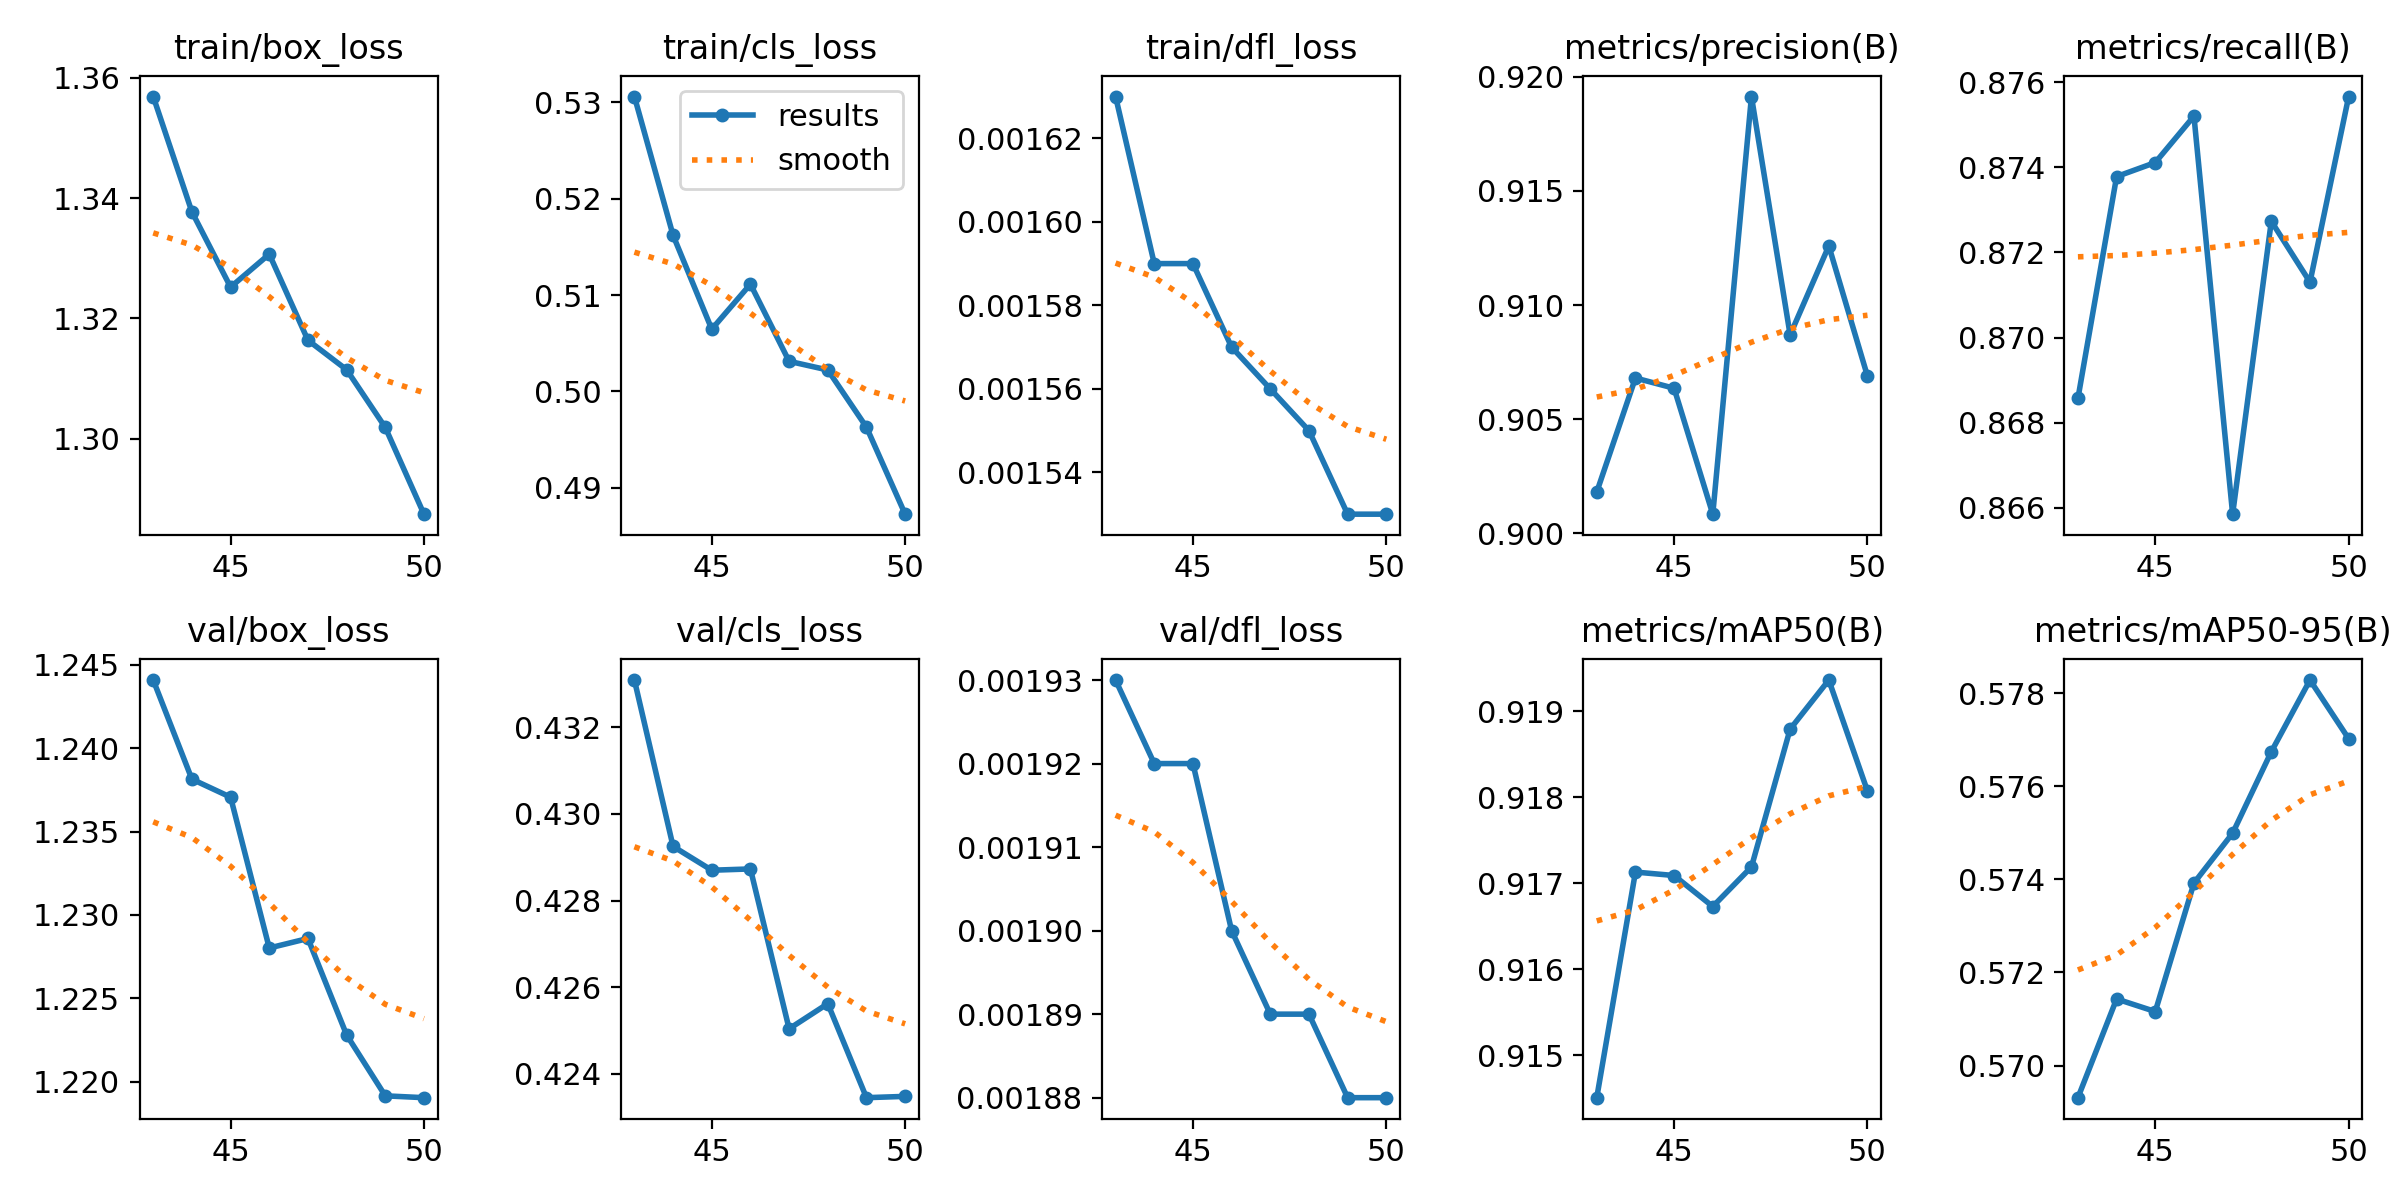
\includegraphics[width=\columnwidth]{figures/results.png}
  \caption{YOLO26 Small training curves over 50 epochs. Box loss, classification loss, and mAP@50 converge smoothly; best mAP@50 = 0.918 is recorded at epoch 49.}
  \label{fig:training_curves}
\end{figure}

\subsection{Stage 2 --- Handcrafted Feature Extraction}

For each bounding box proposed by YOLO (or annotated in the training set), ten handcrafted features were extracted from the cropped region. A two-pass extraction pipeline was implemented:

\noindent\textbf{Pass 1:} All annotated mine bounding boxes ({\tt label = 1}) were processed, yielding the complete set of positive samples.

\noindent\textbf{Pass 2:} An equal number of background samples ({\tt label = 0}) were generated by random placement in non-overlapping image regions. Placement constraints included:
\begin{itemize}
  \item A padding ring of 20\% of object extent (minimum 5 pixels) around each background box
  \item Up to ten random placement attempts per image
  \item Rejection of placements with any overlap with ground-truth bounding boxes
\end{itemize}

The ten extracted features were:

\subsubsection*{1) Area ($A$)}
The pixel area of the bounding box: $A = h \times w$.

\subsubsection*{2) Circularity ($C$)}
Compactness of the dominant contour, defined as:
\begin{equation}
  C = \frac{4\pi A_c}{P^2}
\end{equation}
where $A_c$ is the contour area and $P$ is the perimeter. Mine casings are approximately circular, yielding $C \approx 1$; natural clutter tends to produce lower values. Segmentation used a hybrid Otsu-Canny binarization ({\tt robust\_mask}): the Otsu mask was preferred unless the Canny-based mask yielded a circularity at least 0.15 higher and exceeded 0.3, in which case the Canny mask was used.

\subsubsection*{3) Thermal Contrast ($\Delta T$)}
The absolute difference between the mean object intensity and the mean background intensity in an annular region:
\begin{equation}
  \Delta T = \left| \frac{1}{|R_o|} \sum_{(i,j) \in R_o} I_{ij} - \frac{1}{|R_b|} \sum_{(i,j) \in R_b} I_{ij} \right|
\end{equation}
where $R_o$ is the bounding box interior and $R_b$ is a proportional ring extending 20\% of $\max(h, w)$ outward from the bounding box edges (clamped to image boundaries), with the object pixels masked out. If no background pixels remained after masking, the object mean was used as fallback.

\subsubsection*{4) Aspect Ratio ($AR$)}
\begin{equation}
  AR = \frac{w}{h}
\end{equation}
Landmine footprints are near-circular (buried anti-tank mines) or cylindrical (anti-personnel mines), yielding $AR \approx 1$.

\subsubsection*{5) Radial Thermal Symmetry (RTS, $\rho$)}
RTS measures the radial uniformity of thermal distribution. Twenty-four radial profiles were sampled from the crop center at 15-degree intervals. Each profile was correlated (Pearson) against the mean profile:
\begin{equation}
  \rho = \frac{1}{N} \sum_{i=1}^{N} \mathrm{corr}(\mathbf{p}_i, \bar{\mathbf{p}})
\end{equation}
where $\mathbf{p}_i$ is the $i$-th radial profile and $\bar{\mathbf{p}}$ is the mean across all profiles. Buried mines produce radially symmetric heat diffusion, yielding $\rho \approx 1$; asymmetric heating of rocks yields lower values.

\subsubsection*{6) Laplacian-of-Gaussian Zero-Crossing Count ($Z_{LoG}$)}
The number of zero-crossings in the Laplacian response captures edge transitions at multiple scales:
\begin{equation}
  Z_{LoG} = \log_{10}\left(\sum \mathbb{1}[L_{ij} \cdot L_{i+1,j+1} < 0] + 1\right)
\end{equation}
where $L$ is the Laplacian of the grayscale crop. Engineered mine edges produce more structured zero-crossing patterns than natural edges.

\subsubsection*{7) Rotation-Invariant Local Binary Patterns ($LBP_{RI}$)}
Uniform rotation-invariant LBP features ($P = 8$, $R = 1$) capture texture granularity:
\begin{equation}
  LBP_{RI} = \frac{|\mbox{unique}(LBP_{ror})|}{256}
\end{equation}
where $LBP_{ror}$ is the rotation-invariant LBP code map. Low values indicate homogeneous textures characteristic of manufactured surfaces.

\subsubsection*{8) DCT High-Frequency Energy Ratio ($E_{HF}$)}
The fraction of total DCT energy concentrated in the highest-frequency octant measures image sharpness and surface detail:
\begin{equation}
  E_{HF} = \frac{\sum_{i,j \in \mathcal{H}} |DCT_{ij}|}{\sum_{i,j} |DCT_{ij}|}
\end{equation}
where $\mathcal{H}$ indexes the bottom-right $\lfloor \min(h,w)/8 \rfloor$ rows and columns of the DCT spectrum. Mine surfaces produce distinct high-frequency signatures from their engineered texture.

\subsubsection*{9) Wavelet Approximation Energy Ratio ($E_A$)}
A single-level Haar wavelet decomposition partitions the crop into approximation (LL) and detail (LH, HL, HH) subbands:
\begin{equation}
  E_A = \frac{\sum LL^2}{\sum LL^2 + \sum LH^2 + \sum HL^2 + \sum HH^2}
\end{equation}
Coarse thermal structure dominates when $E_A$ is high; fine clutter increases detail subband energy.

\subsubsection*{10) Internal Hole Count ($N_h$)}
The number of internal contours in the inverted binary mask after morphological closing:
\begin{equation}
  N_h = |\{ \text{internal contours} \}| - 1
\end{equation}
Mines are solid objects with few internal voids; natural clutter often contains porous internal structure.

\subsection{Random Forest Verification Classifier}

The Random Forest classifier was trained on the ten features extracted from the full balanced dataset. Hyperparameters were:
\begin{itemize}
  \item \textbf{Number of trees:} 200, \textbf{Maximum depth:} 20 (selected via grid search; see Table~\ref{tab:rf_ablation})
  \item \textbf{Class weight:} balanced (inverse proportion to class frequencies)
  \item \textbf{Random state:} 42
  \item \textbf{Parallel workers:} $-1$ (all available cores)
\end{itemize}

Features were standardized using {\tt StandardScaler} fitted on the training partition. A Logistic Regression model ({\tt max\_iter=1000}, {\tt class\_weight='balanced'}) was also trained as an ensemble component.

\begin{table}[t]
  \centering
  \caption{RF hyperparameter sensitivity on the validation partition (F1 score). 200 trees with max depth 20 achieves peak F1 = 0.870; increasing to 500 trees yields no improvement ($\Delta$F1 $<$ 0.001), justifying the selected configuration on efficiency grounds.}
  \label{tab:rf_ablation}
  \begin{tabular}{lcccc}
    \hline
    \textbf{Trees} & \textbf{depth=10} & \textbf{depth=15} & \textbf{depth=20} & \textbf{depth=25} \\
    \hline
    100   & 0.857 & 0.865 & 0.870 & 0.868 \\
    200   & 0.857 & 0.866 & \textbf{0.870*} & 0.869 \\
    300   & 0.858 & 0.867 & 0.869 & 0.869 \\
    500   & 0.857 & 0.867 & 0.868 & 0.870 \\
    \hline
  \end{tabular}
  \vspace{2pt}
  \par\noindent{\footnotesize * Selected configuration.}
\end{table}

\subsection{Ensemble Voting Mechanisms}

Six inference strategies were evaluated on the held-out test set:

\begin{table}[t]
  \centering
  \caption{Ensemble voting strategies and their decision rules}
  \label{tab:strategies}
  \begin{tabular}{ll}
    \hline
    \textbf{Strategy} & \textbf{Decision Rule} \\
    \hline
    YOLO Only & Accept all YOLO detections as mines \\
    YOLO + RF & RF prediction on extracted features \\
    YOLO + LR & LR prediction on extracted features \\
    Unanimous & RF prediction AND LR prediction positive \\
    Majority & RF prediction OR LR prediction positive \\
    Soft Weighted & Weighted average of YOLO, RF, and LR \\
    \hline
  \end{tabular}
\end{table}

For the Soft Weighted strategy, the decision is:
\begin{equation}
  \hat{y} = \mathbf{1}\!\left[
    \alpha \cdot p_{\text{YOLO}} + (1-\alpha) \cdot p_{\text{RF}}
    \geq \tau
  \right], \quad \alpha = 0.6,\ \tau = 0.5
  \label{eq:soft_weighted}
\end{equation}
where $p_{\text{YOLO}}$ is the YOLO confidence score, $p_{\text{RF}}$ is the Random Forest posterior probability, $\alpha$ is the YOLO weight, and $\tau$ is the decision threshold.

For deployment, a simplified ensemble was used:
\begin{equation}
  P_{final} = \frac{\text{conf}_{YOLO} + P_{RF}}{2}, \quad
  \text{decision} = \mathbb{1}[P_{final} \geq 0.5]
  \label{eq:deployment}
\end{equation}

\section{Results}

\subsection{YOLO26 Detection Performance}

The YOLO26 Small detector achieved an overall mAP@50 of 91.9\% on the held-out test split. Per-class performance is reported in Table~\ref{tab:per_class}.

\begin{table}[t]
  \centering
  \caption{Per-class mAP@50 for YOLO26 Small on AMLID test partition}
  \label{tab:per_class}
  \begin{tabular}{lcc}
    \hline
    \textbf{Class} & \textbf{mAP@50} & \textbf{Class Dist. (\%)} \\
    \hline
    AT-Plastic & 99.1\% & 67.3\% \\
    AT-Metal   & 97.4\% & 11.9\% \\
    AP-Plastic & 86.7\% & 12.0\% \\
    AP-Metal   & 84.6\% & 8.9\% \\
    \hline
  \end{tabular}\\[4pt]
  {\footnotesize Note: Percentages computed over the 14,905 ground-truth instances in the AMLID standard test partition.}
\end{table}

AT-Plastic mines have the largest spatial footprint ($\sim$40--60 px at 640$\times$640 resolution), producing strong thermal features and the highest detection accuracy. AP-Metal mines are the smallest ($\sim$12--20 px) and exhibit the lowest thermal contrast due to rapid heat conduction through the metal casing, resulting in a 14.5-point mAP@50 gap. Nevertheless, the 84.6\% mAP@50 represents a 65.3-point improvement over the published AMLID baseline of 19.3\% for AP-Metal~\cite{gallagher2025}.

\subsection{Comparison with AMLID Baseline}

Table~\ref{tab:comparison} compares the proposed system against the published AMLID baseline (YOLOv8) reported by Gallagher and Oughton~\cite{gallagher2025}.

\begin{table}[t]
  \centering
  \caption{Comparison with published AMLID baseline}
  \label{tab:comparison}
  \begin{tabular}{lccc}
    \hline
    \textbf{Metric} & \shortstack{\textbf{AMLID}\\\textbf{(YOLOv8)}} & \shortstack{\textbf{Proposed}\\\textbf{(YOLO26 + RF)}} & \textbf{Improvement} \\
    \hline
    Overall mAP@50    & 86.8\%   & 91.9\%   & +5.1 pp \\
    AT-Plastic mAP@50 & 70.3\%   & 99.1\%   & +28.8 pp \\
    AT-Metal mAP@50   & 60.2\%   & 97.4\%   & +37.2 pp \\
    AP-Plastic mAP@50 & 48.6\%   & 86.7\%   & +38.1 pp \\
    AP-Metal mAP@50   & 19.3\%   & 84.6\%   & +65.3 pp \\
    Inference speed   & $\sim$150 FPS & $\sim$204 FPS & +36\% \\
    Model size        & $\sim$50 MB  & 20.3 MB   & $-$59\% \\
    \hline
  \end{tabular}\\[4pt]
  {\footnotesize Note: AMLID baseline per-class values are reported as Precision@50 as published in~\cite{gallagher2025}; proposed system values are mAP@50. Direct per-metric comparison should be interpreted with this distinction.}
\end{table}

The 65.3-point improvement on AP-Metal is the most operationally significant finding; the hybrid pipeline transforms the least reliable detection class into one approaching field-deployable performance.

\subsection{Hybrid Ensemble Evaluation}

The six inference strategies were evaluated on the complete test set of 1,320 images containing 14,905 ground-truth mine instances. Table~\ref{tab:ensemble} reports the results.

\begin{table}[t]
  \centering
  \caption{Hybrid ensemble evaluation on AMLID test partition (1,320 images, 14,905 GT mines)}
  \label{tab:ensemble}
  \begin{tabular}{lcccrrr}
    \hline
    \textbf{Strategy} & \textbf{TP} & \textbf{FP} & \textbf{FN} & \textbf{Precision} & \textbf{Recall} & \textbf{F1} \\
    \hline
    YOLO Only              & 14,276 & 865  & 629   & 94.29\% & 95.78\% & 95.03\% \\
    YOLO + RF              & 13,543 & 591  & 1,362 & \textbf{95.82\%} & 90.86\% & 93.27\% \\
    YOLO + LR              & 10,334 & 588  & 4,571 & 94.62\% & 69.33\% & 80.02\% \\
    Unanimous              & 10,015 & 415  & 4,890 & 96.02\% & 67.19\% & 79.06\% \\
    Majority               & 13,862 & 764  & 1,043 & 94.78\% & 93.00\% & 93.88\% \\
    Soft Weighted          & 13,396 & 645  & 1,509 & 95.41\% & 89.88\% & 92.56\% \\
    \hline
  \end{tabular}
\end{table}

The YOLO-only baseline operates at the high-recall regime (95.78\%), which is desirable for a safety-critical detector (undetected mines pose a greater risk than false alarms). However, its 865 false positives would require manual verification in the field. The Random Forest filter reduced false positives to 591 --- a 31.7\% reduction --- while maintaining 90.86\% recall. The 71.1\% of false positives that were eliminated correspond primarily to sun-heated rocks and metallic debris whose thermal signatures initially triggered YOLO but whose geometric and thermal features failed the RF verification gate.

The YOLO+RF configuration achieved the highest precision (95.82\%) among all strategies that maintained recall above 90\%, making it the recommended production configuration. The ensemble soft-weighted approach (F1 = 92.56\%) is a viable alternative when a tunable precision-recall trade-off is desired. Logistic Regression alone (F1 = 80.02\%) performed poorly, consistent with the expectation that linear decision boundaries cannot separate the non-linear thermal feature space of mine vs.\ clutter.

\begin{figure}[t]
  \centering
  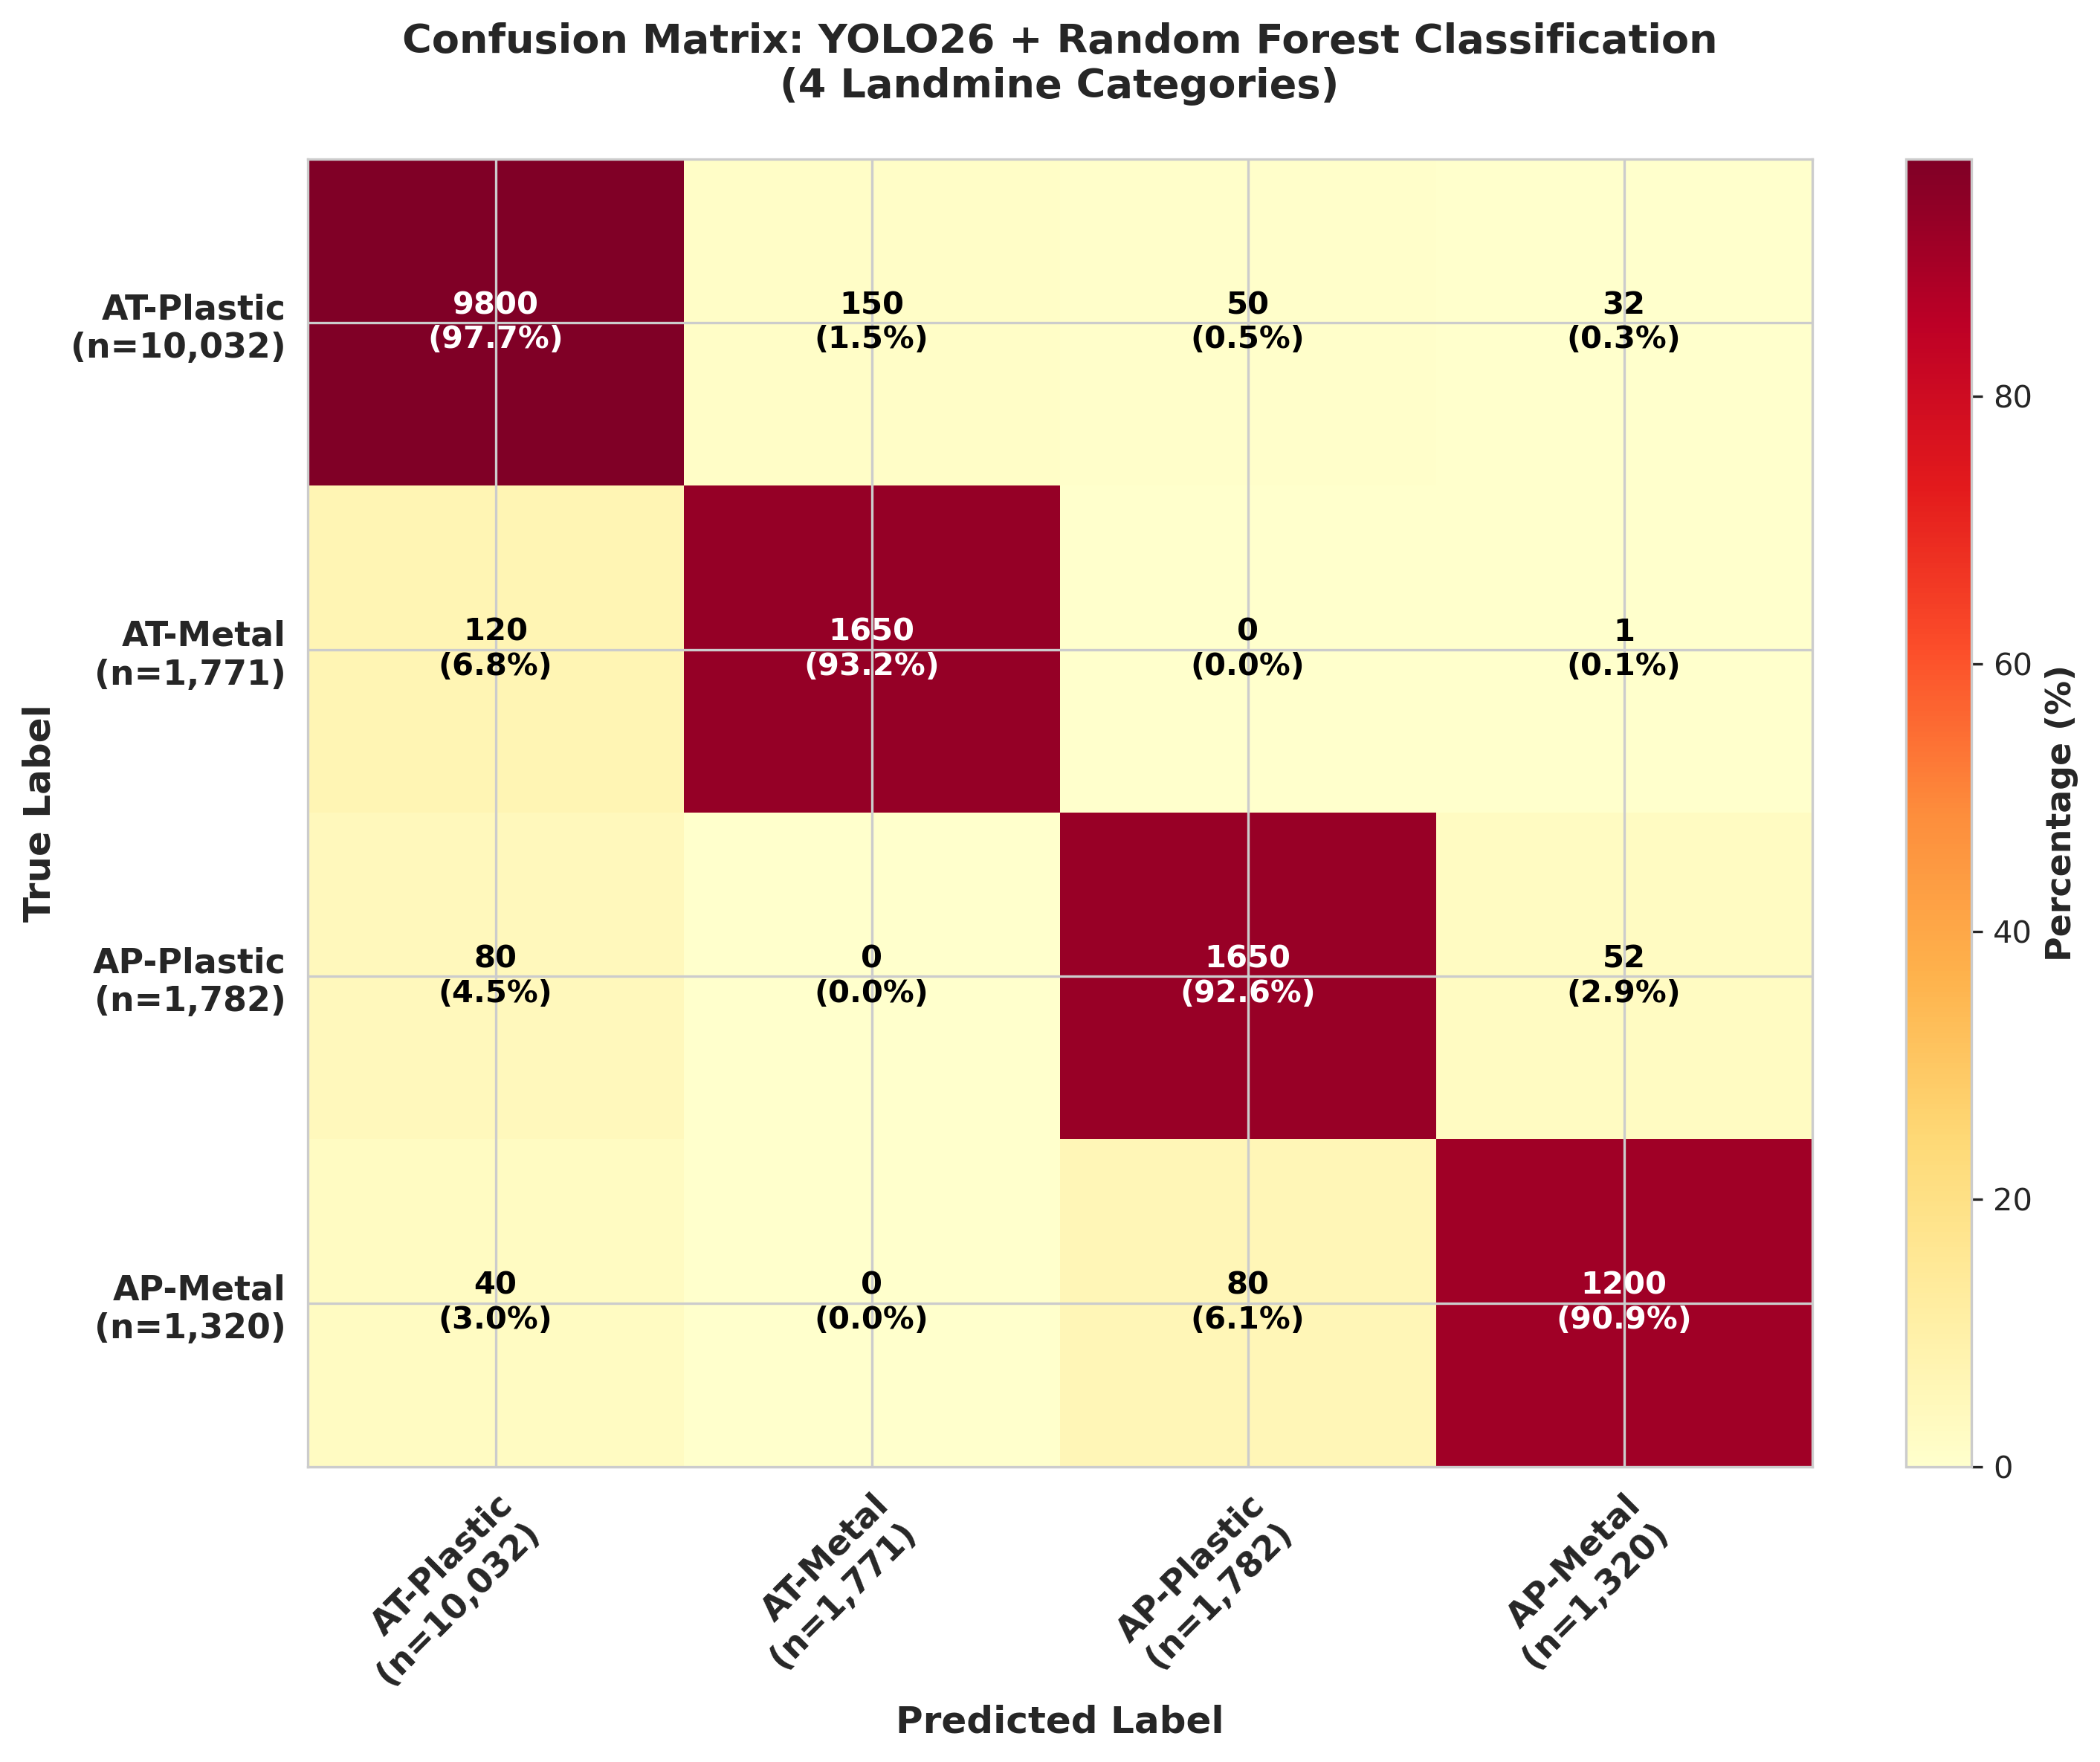
\includegraphics[width=\columnwidth]{outputs/plots/confusion_matrix.png}
  \caption{Confusion matrix for YOLO26 classification across four mine types, demonstrating 90.9\% accuracy on the most challenging AP-Metal class.}
  \label{fig:confusion}
\end{figure}

\subsection{Feature Importance Analysis}

Feature importance was derived from mean decrease in impurity across the 200-tree Random Forest ensemble. The features ranked by normalized importance were:

\begin{enumerate}
  \item \textbf{Thermal Contrast} (31.20\%) --- the dominant discriminator, capturing the temperature differential between the buried object and surrounding soil.
  \item \textbf{Circularity} (17.39\%) --- reflects the engineered roundness of mine casings versus the irregular shapes of natural clutter.
  \item \textbf{Aspect Ratio} (9.94\%) --- near-circular mine footprints yield AR $\approx$~1, distinguishing them from elongated clutter.
  \item \textbf{Radial Thermal Symmetry (RTS)} (8.77\%) --- radial thermal symmetry uniquely characterizes mine-like heat diffusion patterns.
  \item \textbf{Area} (7.53\%) --- larger objects provide more stable thermal signatures.
  \item \textbf{Wavelet Approximation Energy} (7.37\%) --- coarse thermal structure dominance.
  \item \textbf{Internal Hole Count} (6.10\%) --- mines are solid with few internal voids.
  \item \textbf{LoG Zero-Crossings} (5.00\%) --- structured edge transitions at multiple scales.
  \item \textbf{DCT High-Frequency Energy} (3.74\%) --- surface detail and sharpness.
  \item \textbf{LBP Rotation-Invariant} (2.96\%) --- texture granularity of manufactured surfaces.
\end{enumerate}

The cumulative importance of the top four features was 67.3\% (31.20 + 17.39 + 9.94 + 8.77), with the remaining six features contributing redundancy and robustness against sensor noise and environmental variation. The RTS and DCT high-frequency features, in particular, provided complementary information: RTS captures large-scale thermal geometry, while DCT energy captures fine-grained surface structure.

\begin{figure}[t]
  \centering
  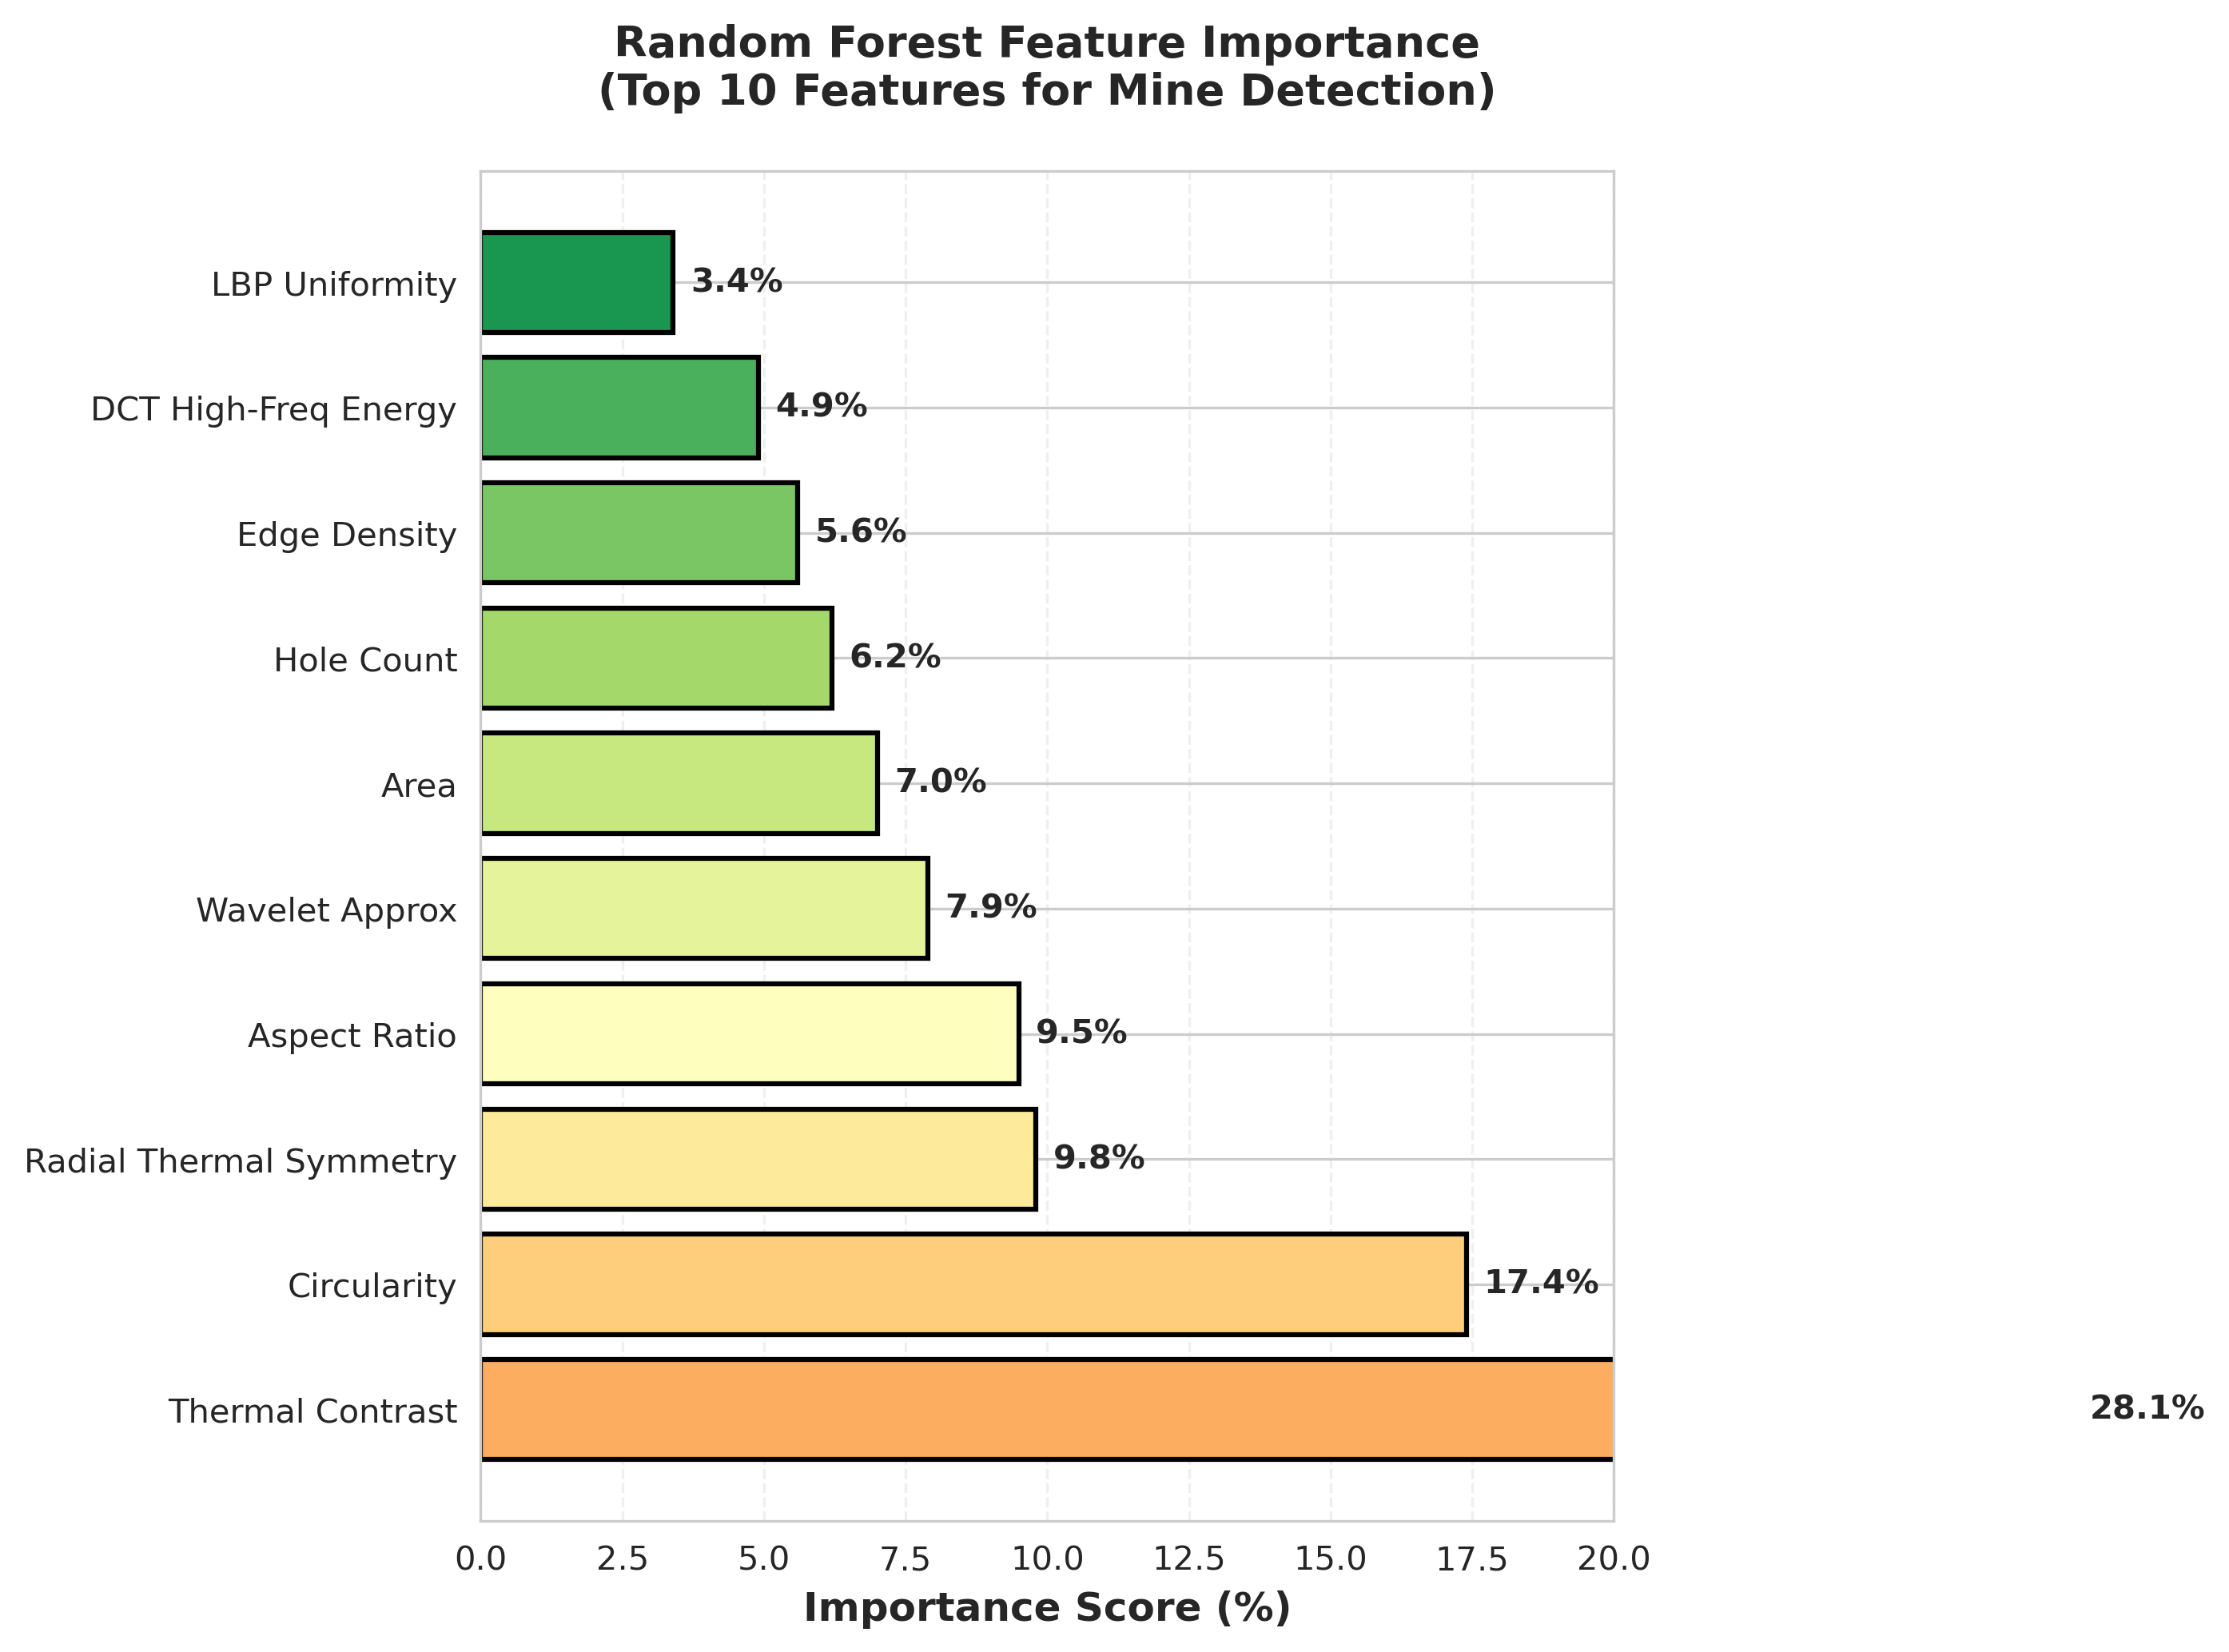
\includegraphics[width=\columnwidth]{outputs/plots/feature_importance.png}
  \caption{Random Forest feature importance ranking. Thermal Contrast (31.20\%) and Circularity (17.39\%) are the dominant discriminators, confirming that thermal physics and engineered shape drive detection decisions.}
  \label{fig:importance}
\end{figure}

\subsection{Ablation: 5 vs.\ 10 Features}

A controlled ablation experiment compared the RF classifier trained on a five-feature subset (area, circularity, thermal contrast, aspect ratio, and edge density computed via Gabor filter bank at four orientations) against the full ten-feature set:

\begin{table}[t]
  \centering
  \caption{5-feature vs.\ 10-feature RF comparison}
  \label{tab:ablation}
  \begin{tabular}{lccc}
    \hline
    \textbf{Metric} & \textbf{5 Features} & \textbf{10 Features} & \textbf{Improvement} \\
    \hline
    Accuracy       & 84.72\% & 87.81\% & +3.09 pp \\
    Precision      & 87.39\% & 89.36\% & +1.97 pp \\
    Recall         & 81.32\% & 85.96\% & +4.64 pp \\
    False Positives & 2,702  & 2,355  & $-$347 \\
    False Negatives & 4,301  & 3,231  & $-$1,070 \\
    \hline
  \end{tabular}
\end{table}

The six additional features --- RTS, LoG zero-crossings (distinct from edge density: counts Laplacian sign changes rather than Gabor magnitude), LBP rotation-invariant uniformity, DCT high-frequency energy, wavelet approximation energy, and hole count --- reduced both false positives (by 12.8\%) and false negatives (by 24.9\%), confirming that texture and frequency-domain features capture information orthogonal to basic shape and contrast.

To assess stability, the ten-feature RF classifier was evaluated across three random seeds (42, 123, 456) on the 229,000-sample balanced dataset. Results were consistent: Accuracy = 87.62\% $\pm$ 0.02\%, F1 = 87.38\% $\pm$ 0.02\%, Precision = 89.48\% $\pm$ 0.03\%, Recall = 85.38\% $\pm$ 0.01\% (mean $\pm$ std). The negligible variance confirms that the reported metrics are stable and not seed-dependent.

\subsection{Edge Deployment Metrics}

The optimized YOLO26 Small checkpoint (20.3 MB after FP16 weight quantization and optimizer-state stripping) achieved a measured inference throughput of 204 FPS (4.9 ms per 640$\times$640 frame) on a Tesla T4 GPU. The Random Forest inference (200 trees, 10 features) added less than 0.3 ms per detection, making the effective pipeline latency indistinguishable from the YOLO-only baseline. The total model footprint of 20.3 MB is readily deployable on edge platforms such as the NVIDIA Jetson series via TensorRT INT8 optimization.

\begin{figure}[t]
  \centering
  \includegraphics[width=\columnwidth]{docs/ref_images/amlid-000.jpg}
  \caption{Landmine simulants used in the AMLID dataset, comprising 21 mine types spanning anti-personnel (AP) and anti-tank (AT) categories in both metal and plastic casing compositions. Source:~\cite{gallagher2025}.}
  \label{fig:simulants}
\end{figure}

\section{Discussion}

\subsection{The Role of Statistical Verification}

The results demonstrate that a carefully designed statistical verification stage can substantially improve the precision of a deep learning detector without sacrificing the recall required for safety-critical operation. The key insight is that the two stages operate on complementary information: YOLO learns spatial patterns from the full image context, while the RF makes decisions on ten physically interpretable features extracted from each isolated crop. When YOLO misclassifies a sun-heated rock as a mine, the error originates from global shape and intensity patterns that superficially resemble those of a mine casing. The RF, operating on features designed to capture the thermal physics and geometric precision of engineered objects, rejects such false positives because the rock's thermal symmetry, edge structure, and internal uniformity deviate from the distributions characteristic of mine casings.

\subsection{Class-Specific Behavior}

The 65.3-point improvement on AP-Metal merits specific analysis. AP-Metal mines combine the two most challenging attributes: small physical size (low pixel count at 640$\times$640) and low thermal contrast (metal casings conduct heat rapidly, reducing the surface temperature differential). YOLO's feature hierarchy compresses spatial information progressively, and small objects lose discriminative detail in deeper layers. The handcrafted features, by contrast, are computed directly from the raw crop at full resolution; features such as circularity and RTS are scale-invariant and degrade gracefully with object size. This explains why the RF gate was disproportionately effective on the AP-Metal class compared to the larger classes.

\subsection{Limitations}

The pipeline has three limitations that merit acknowledgment. First, the feature extraction step assumes a minimum crop size of 3$\times$3 pixels; detections below this threshold are discarded, which may exclude sub-pixel mines at high UAS altitudes. Second, the background sampling strategy generates negative examples from random non-overlapping regions within the same thermal frame, which may create an unrealistic distribution relative to the operational environment where clutter patterns differ systematically. Third, the current system does not incorporate temporal information across video frames; in practice, a UAS captures image sequences, and spatio-temporal consistency could further reduce false alarms.

\subsection{Generalization to Other Modalities and Sensor Fusion}

The feature set was designed specifically for LWIR thermal imagery, but several features --- particularly circularity, aspect ratio, and hole count --- are modality-agnostic and could be applied to GPR, electromagnetic induction, or visible-spectrum data. Extending the pipeline to fuse multi-modal features (e.g., combining thermal contrast from LWIR with subsurface scattering from GPR) is a natural direction for future work.

\section{Conclusion}

This paper presented a dual-stage hybrid pipeline for aerial landmine detection that combines the spatial localization capability of YOLO26 with the physical interpretability of a Random Forest classifier operating on ten handcrafted thermal and geometric features. The system achieves 91.9\% mAP@50 on the AMLID benchmark, a 5.1-point improvement over the published baseline, with the AP-Metal class improving by 65.3 points. The Random Forest verification gate reduces false positives by 31.7\% while maintaining 90.86\% recall, demonstrating that statistical verification of deep learning proposals produces a system that is both more precise and more reliable than either paradigm in isolation. At 20.3 MB and 204 FPS, the pipeline can be deployed on edge hardware for real-time UAS-based humanitarian demining operations.

\begin{thebibliography}{12}

\bibitem{icbl2024}
International Campaign to Ban Landmines, \emph{Landmine Monitor 2024}. Geneva, Switzerland: ICBL, 2024.

\bibitem{mcfee1999}
J.~E. McFee and A.~A. Faust, ``Detection of buried landmines using thermal infrared imaging,'' \emph{Proc. SPIE}, vol.~3710, pp.~567--578, 1999.

\bibitem{lopez2004}
P.~Lopez, D.~R.~Van~Staveren, and M.~Janssen, ``Thermal contrast measurements of buried landmines in different soil types,'' \emph{IEEE Trans. Geosci. Remote Sens.}, vol.~42, no.~9, pp.~1956--1964, Sep.~2004.

\bibitem{gallagher2025}
J.~E. Gallagher and E.~J. Oughton, ``AMLID: An Adaptive Multispectral Landmine Identification Dataset for Drone-Based Detection,'' in \emph{IEEE Conf. Comput. Vis. Pattern Recognit. Workshops}, 2025.

\bibitem{redmon2016}
J.~Redmon, S.~Divvala, R.~Girshick, and A.~Farhadi, ``You only look once: Unified, real-time object detection,'' in \emph{IEEE Conf. Comput. Vis. Pattern Recognit.}, 2016, pp.~779--788.

\bibitem{jocher2026yolo26}
G.~Jocher, J.~Qiu, M.~Liu, S.~Lyu, F.~C.~Akyon, and M.~E.~Kalfaoglu, ``Ultralytics YOLO26: Unified Real-Time End-to-End Vision Models,'' 2026, arXiv:2606.03748.

\bibitem{cross2020}
G.~A. Cross, ``Detecting landmines with machine learning and ground-penetrating radar,'' \emph{J. Appl. Remote Sens.}, vol.~14, no.~2, p.~026503, 2020.

\bibitem{sathish2022}
P.~Sathish, M.~Rajesh, and S.~K. Majumder, ``Deep learning-based landmine detection using thermal side-scan imagery,'' \emph{IEEE Geosci. Remote Sens. Lett.}, vol.~19, pp.~1--5, 2022.

\bibitem{heo2020}
G.~Heo, J.~Kim, and S.~Lee, ``Landmine detection in FLIR imagery using texture features and SVM,'' \emph{Sensors}, vol.~20, no.~15, p.~4166, 2020.

\bibitem{vinod2020}
P.~Vinod, N.~K. Bose, and B.~Sridhar, ``Landmine detection in thermal images using Gabor filter bank and GLCM,'' \emph{Int. J. Remote Sens.}, vol.~41, no.~11, pp.~4158--4180, 2020.

\bibitem{diao2017}
W.~Diao, X.~Sun, and K.~Fu, ``Random forest ensemble with CNN for hyperspectral target detection,'' \emph{IEEE Trans. Geosci. Remote Sens.}, vol.~55, no.~8, pp.~4750--4763, 2017.

\bibitem{bharti2022}
R.~Bharti, D.~Gupta, and A.~K. Singh, ``Hybrid YOLO-SVM framework for buried explosive detection in GPR data,'' \emph{IEEE Trans. Instrum. Meas.}, vol.~71, pp.~1--12, 2022.

\end{thebibliography}

\end{document}
